% =====================================================================
%  8. PROPUESTA DE PLAN DE MEJORA CONTINUA (PHVA)
%  Responsable: INTEGRANTE 5
%  Extensión objetivo: 6 a 8 páginas — aprox. 2.400 palabras + Tabla 4 + Figura 4
%
%  ESTA ES LA EVIDENCIA EVI. 6 PROPIAMENTE DICHA.
%
%  REGLA QUE DISTINGUE UN TRABAJO DE NOTA ALTA:
%  cada acción que propongas debe estar MAPEADA a (a) un hallazgo concreto
%  de la sección 6 y (b) un requisito concreto de IFC PS, GISTM o IRMA.
%  Si una acción no se puede mapear a ninguno de los dos, sobra.
%
%  Y cada acción debe ser verificable: responsable, plazo, indicador y meta.
%  «Mejorar la relación con la comunidad» no es una acción, es un deseo.
% =====================================================================

\section{Propuesta de plan de mejora continua}

% ---------------------------------------------------------------------
\subsection{Política y compromiso}
% Extensión: ~0,75 página / 280 palabras

% TODO: Redacta la política ambiental y social que debería adoptar la
%   operación, con los elementos que exige ISO 14001:2015: compromiso de
%   protección del ambiente, de cumplimiento de requisitos legales y otros
%   requisitos, y de mejora continua. Añade los compromisos específicos que
%   el caso reclama: respeto a los derechos de los pueblos indígenas,
%   consulta previa, y adhesión expresa a los VPSHR.
%   Fuentes: \cite{iso2015iso14001}, \cite{vpshr2000principios}

% ---------------------------------------------------------------------
\subsection{Planificar}
% Extensión: ~1,5 páginas / 550 palabras

% TODO: - Identificación de ASPECTOS e IMPACTOS ambientales y sociales, con
%         criterio de significancia declarado. Aspectos que el caso exige
%         incluir: uso y manejo de cianuro; generación y depósito de
%         relaves; potencial de drenaje ácido de roca; captación y descarga
%         de agua; subsidencia por labores subterráneas; adquisición de
%         tierras; y presencia de seguridad armada.
%       - Identificación de requisitos legales y otros requisitos (aquí
%         entran el Convenio 169, los IFC PS por el préstamo, y el GISTM).
%       - Objetivos y metas MEDIBLES derivados de los hallazgos de la
%         sección 6. Un objetivo por hallazgo central, como mínimo.
%       - Análisis de partes interesadas: comunidades de San Miguel
%         Ixtahuacán y Sipacapa, autoridades indígenas, Estado, IFC,
%         accionistas, trabajadores y ONG.
%       Fuentes: \cite{iso2015iso14001}, \cite{icmm2020gistm}

% ---------------------------------------------------------------------
\subsection{Hacer}
% Extensión: ~1,5 páginas / 550 palabras

% TODO: - Controles operacionales: gestión de cianuro conforme al
%         International Cyanide Management Code; gestión de relaves conforme
%         al GISTM (recuerda: el GISTM es de 2020, así que aquí lo propones
%         como estándar de referencia actual, no como norma que la operación
%         incumplió en su momento); monitoreo de calidad de agua con cadena
%         de custodia y laboratorio acreditado.
%       - PROGRAMA DE RELACIONAMIENTO COMUNITARIO con proceso de consulta
%         previa, libre e informada conforme al Convenio 169 y al IFC PS7.
%       - MECANISMO DE QUEJAS Y RECLAMOS con criterios de eficacia
%         (legítimo, accesible, predecible, equitativo, transparente,
%         compatible con derechos y fuente de aprendizaje continuo).
%         Responde directamente al hallazgo central 4 de la sección 6.
%       - Adopción formal de los VPSHR: capacitación de la seguridad privada,
%         reglas de uso de la fuerza, y registro y reporte de incidentes.
%       - Competencia, formación y toma de conciencia del personal.
%       Fuentes: \cite{oit1989convenio169}, \cite{vpshr2000principios}, \cite{ifcsfmarlin}

% ---------------------------------------------------------------------
\subsection{Verificar}
% Extensión: ~1,25 páginas / 450 palabras

% TODO: - MONITOREO PARTICIPATIVO: es la pieza clave y hay dos modelos
%         citables en la propia bitácora — la AMAC (Asociación de Monitoreo
%         Ambiental Comunitario) del propio caso Marlin, y la mesa de
%         diálogo de Espinar con su Monitoreo Sanitario Ambiental
%         Participativo de 2013 (313 puntos de monitoreo y 40 sustancias
%         analizadas por punto). Usa Espinar como referencia de diseño
%         técnico: es el ejemplo de escala que da credibilidad.
%         \cite{minam2013espinar}
%       - Indicadores y su periodicidad de medición.
%       - Programa de AUDITORÍAS INTERNAS conforme a ISO 19011:2018.
%         \cite{iso2018iso19011}
%       - Verificación independiente de tercera parte: aquí propón el
%         estándar IRMA, que exige al menos 90 % de cumplimiento en cada una
%         de sus cuatro áreas de principios y auditoría independiente.
%         \cite{irmasfstandard}
%       - Revisión quinquenal de seguridad de la presa de relaves.

% ---------------------------------------------------------------------
\subsection{Actuar}
% Extensión: ~1 página / 380 palabras

% TODO: - Tratamiento de no conformidades y acciones correctivas: análisis
%         de causa raíz, no solo corrección del síntoma.
%       - Criterio de CIERRE de una no conformidad: cuándo se considera
%         efectivamente cerrada y quién lo verifica.
%       - Revisión por la dirección: entradas, salidas y periodicidad.
%       - Retroalimentación al ciclo: cómo los resultados del monitoreo
%         participativo modifican los objetivos de la fase Planificar.
%       - Gestión del cierre y post-cierre, que en este caso es la fase
%         realmente pendiente: la mina cerró en 2017 y el post-cierre es
%         donde se juega el pasivo de largo plazo.
%       Fuentes: \cite{iso2015iso14001}, \cite{goldcorp2023marlin}

% ---------------------------------------------------------------------
\subsection{Matriz del plan de acción}
% Extensión: Tabla 4 (2 páginas apaisadas) + ~200 palabras de lectura

% --- TABLA 4: Plan de acción -----------------------------------------
% Una fila por acción. Mínimo dos acciones por cada uno de los siete ejes.
% La columna «Estándar de referencia» es la que demuestra el mapeo exigido.
%\begin{landscape}
%\begin{footnotesize}
%\begin{longtable}{@{}L{3.5cm} L{4.5cm} L{2.5cm} L{2cm} L{3.5cm} L{2.5cm} L{2.5cm}@{}}
%  \caption{Plan de acción para la mejora continua de la gestión socioambiental}
%  \label{tab:plan-accion} \\
%  \toprule
%  \textbf{Objetivo} & \textbf{Acción} & \textbf{Responsable} & \textbf{Plazo} & \textbf{Indicador} & \textbf{Meta} & \textbf{Recursos} \\
%  \midrule
%  \endfirsthead
%  \multicolumn{7}{l}{\footnotesize\textit{Tabla \ref{tab:plan-accion} (continuación)}} \\
%  \toprule
%  \textbf{Objetivo} & \textbf{Acción} & \textbf{Responsable} & \textbf{Plazo} & \textbf{Indicador} & \textbf{Meta} & \textbf{Recursos} \\
%  \midrule
%  \endhead
%  \bottomrule
%  \multicolumn{7}{l}{\footnotesize Nota. Elaboración propia.} \\
%  \endlastfoot
%   & & & & & & \\
%   & & & & & & \\
%\end{longtable}
%\end{footnotesize}
%\end{landscape}

% ---------------------------------------------------------------------
\subsection{Mapeo de recomendaciones de la auditoría a estándares internacionales}
% Extensión: ~0,75 página / 280 palabras

% TODO: Tabla o lista que cruce cada recomendación de la HRIA con el
%   requisito concreto que la respalda. Ejemplos para arrancar:
%     Consulta previa            -> Convenio 169 OIT art. 6 + IFC PS7
%     Monitoreo de agua          -> IFC PS3 + GISTM Tema III
%     Gestión de relaves         -> GISTM (15 principios, 77 requisitos auditables)
%     Seguridad privada          -> VPSHR + IFC PS4
%     Adquisición de tierras     -> IFC PS5
%     Mecanismo de quejas        -> IFC PS1 + marco Ruggie, pilar «Remediar»
%     Verificación independiente -> IRMA
%   Fuentes: \cite{icmm2020gistm}, \cite{irmasfstandard}, \cite{ifcsfmarlin}

% --- FIGURA 4: Ciclo PHVA aplicado al caso ---------------------------
% Sugerencia: círculo de cuatro cuadrantes, y en cada cuadrante las 3 o 4
% acciones principales que le corresponden en este caso concreto.
% Dibújalo en TikZ o expórtalo a PDF en imagenes/diagramas/.
%\begin{figure}[H]
%  \centering
%  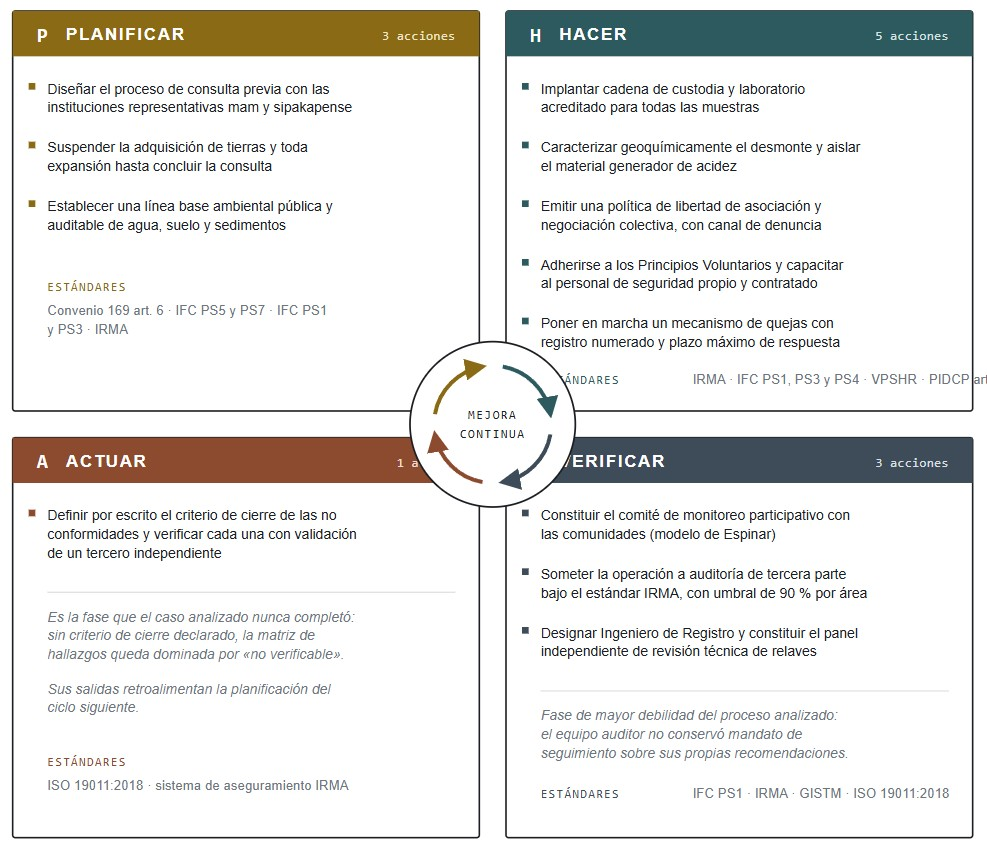
\includegraphics[width=0.8\textwidth]{imagenes/diagramas/ciclo_phva.pdf}
%  \caption{Ciclo PHVA aplicado a la gestión socioambiental de la Mina Marlin}
%  \label{fig:phva}
%  \footnotesize Nota. Elaboración propia a partir de \textcite{iso2015iso14001}.
%\end{figure}

\pendiente{desarrollar la sección 8 (6--8 páginas) + Tabla 4 + Figura 4}
